

\tikzset{every picture/.style={line width=0.75pt}} %set default line width to 0.75pt        

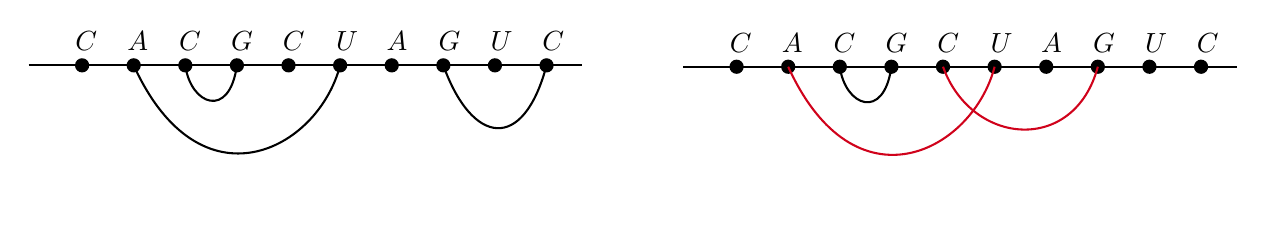
\begin{tikzpicture}[x=0.5pt,y=0.5pt,yscale=-1,xscale=1]
%uncomment if require: \path (0,125); %set diagram left start at 0, and has height of 125

%Flowchart: Connector [id:dp8000065927198341] 
\draw  [fill={rgb, 255:red, 0; green, 0; blue, 0 }  ,fill opacity=1 ] (49,43.9) .. controls (49.87,41.65) and (52.4,40.52) .. (54.66,41.39) .. controls (56.91,42.26) and (58.04,44.79) .. (57.17,47.05) .. controls (56.3,49.3) and (53.77,50.43) .. (51.51,49.56) .. controls (49.26,48.69) and (48.13,46.16) .. (49,43.9) -- cycle ;
%Flowchart: Connector [id:dp15246894411278777] 
\draw  [fill={rgb, 255:red, 0; green, 0; blue, 0 }  ,fill opacity=1 ] (86.3,43.9) .. controls (87.16,41.65) and (89.7,40.52) .. (91.95,41.39) .. controls (94.21,42.26) and (95.33,44.79) .. (94.46,47.05) .. controls (93.59,49.3) and (91.06,50.43) .. (88.81,49.56) .. controls (86.55,48.69) and (85.43,46.16) .. (86.3,43.9) -- cycle ;
%Flowchart: Connector [id:dp36869196941163607] 
\draw  [fill={rgb, 255:red, 0; green, 0; blue, 0 }  ,fill opacity=1 ] (123.59,43.9) .. controls (124.46,41.65) and (126.99,40.52) .. (129.25,41.39) .. controls (131.5,42.26) and (132.63,44.79) .. (131.76,47.05) .. controls (130.89,49.3) and (128.36,50.43) .. (126.1,49.56) .. controls (123.85,48.69) and (122.72,46.16) .. (123.59,43.9) -- cycle ;
%Flowchart: Connector [id:dp16694338209837356] 
\draw  [fill={rgb, 255:red, 0; green, 0; blue, 0 }  ,fill opacity=1 ] (160.89,43.9) .. controls (161.75,41.65) and (164.29,40.52) .. (166.54,41.39) .. controls (168.8,42.26) and (169.92,44.79) .. (169.05,47.05) .. controls (168.18,49.3) and (165.65,50.43) .. (163.4,49.56) .. controls (161.14,48.69) and (160.02,46.16) .. (160.89,43.9) -- cycle ;
%Flowchart: Connector [id:dp42963486447916044] 
\draw  [fill={rgb, 255:red, 0; green, 0; blue, 0 }  ,fill opacity=1 ] (198.18,43.9) .. controls (199.05,41.65) and (201.58,40.52) .. (203.84,41.39) .. controls (206.09,42.26) and (207.22,44.79) .. (206.35,47.05) .. controls (205.48,49.3) and (202.95,50.43) .. (200.69,49.56) .. controls (198.44,48.69) and (197.31,46.16) .. (198.18,43.9) -- cycle ;
%Flowchart: Connector [id:dp5506217339056906] 
\draw  [fill={rgb, 255:red, 0; green, 0; blue, 0 }  ,fill opacity=1 ] (235.48,43.9) .. controls (236.34,41.65) and (238.88,40.52) .. (241.13,41.39) .. controls (243.39,42.26) and (244.51,44.79) .. (243.64,47.05) .. controls (242.77,49.3) and (240.24,50.43) .. (237.99,49.56) .. controls (235.73,48.69) and (234.61,46.16) .. (235.48,43.9) -- cycle ;
%Flowchart: Connector [id:dp9698798449909987] 
\draw  [fill={rgb, 255:red, 0; green, 0; blue, 0 }  ,fill opacity=1 ] (272.77,43.9) .. controls (273.64,41.65) and (276.17,40.52) .. (278.43,41.39) .. controls (280.68,42.26) and (281.81,44.79) .. (280.94,47.05) .. controls (280.07,49.3) and (277.54,50.43) .. (275.28,49.56) .. controls (273.03,48.69) and (271.9,46.16) .. (272.77,43.9) -- cycle ;
%Flowchart: Connector [id:dp6216415603842047] 
\draw  [fill={rgb, 255:red, 0; green, 0; blue, 0 }  ,fill opacity=1 ] (310.07,43.9) .. controls (310.93,41.65) and (313.47,40.52) .. (315.72,41.39) .. controls (317.98,42.26) and (319.1,44.79) .. (318.23,47.05) .. controls (317.36,49.3) and (314.83,50.43) .. (312.58,49.56) .. controls (310.32,48.69) and (309.2,46.16) .. (310.07,43.9) -- cycle ;
%Flowchart: Connector [id:dp3011581402055178] 
\draw  [fill={rgb, 255:red, 0; green, 0; blue, 0 }  ,fill opacity=1 ] (347.36,43.9) .. controls (348.23,41.65) and (350.76,40.52) .. (353.02,41.39) .. controls (355.27,42.26) and (356.4,44.79) .. (355.53,47.05) .. controls (354.66,49.3) and (352.13,50.43) .. (349.87,49.56) .. controls (347.62,48.69) and (346.49,46.16) .. (347.36,43.9) -- cycle ;
%Flowchart: Connector [id:dp9886740109361196] 
\draw  [fill={rgb, 255:red, 0; green, 0; blue, 0 }  ,fill opacity=1 ] (384.66,43.9) .. controls (385.52,41.65) and (388.06,40.52) .. (390.31,41.39) .. controls (392.57,42.26) and (393.69,44.79) .. (392.82,47.05) .. controls (391.95,49.3) and (389.42,50.43) .. (387.17,49.56) .. controls (384.91,48.69) and (383.79,46.16) .. (384.66,43.9) -- cycle ;
%Straight Lines [id:da7380690811587965] 
\draw    (14.5,45.48) -- (414.5,45.48) ;
%Curve Lines [id:da5249448376389138] 
\draw    (90.38,45.48) .. controls (138.5,151) and (223.5,107) .. (239.56,45.48) ;
%Curve Lines [id:da6743430437445295] 
\draw    (127.67,45.48) .. controls (131.5,74) and (159.5,85) .. (164.97,45.48) ;
%Curve Lines [id:da22021299625417579] 
\draw    (314.15,45.48) .. controls (334.8,103) and (371.8,109) .. (388.74,45.48) ;
%Flowchart: Connector [id:dp9581421618036173] 
\draw  [fill={rgb, 255:red, 0; green, 0; blue, 0 }  ,fill opacity=1 ] (522,44.9) .. controls (522.87,42.65) and (525.4,41.52) .. (527.66,42.39) .. controls (529.91,43.26) and (531.04,45.79) .. (530.17,48.05) .. controls (529.3,50.3) and (526.77,51.43) .. (524.51,50.56) .. controls (522.26,49.69) and (521.13,47.16) .. (522,44.9) -- cycle ;
%Flowchart: Connector [id:dp7201955285984009] 
\draw  [fill={rgb, 255:red, 0; green, 0; blue, 0 }  ,fill opacity=1 ] (559.3,44.9) .. controls (560.16,42.65) and (562.7,41.52) .. (564.95,42.39) .. controls (567.21,43.26) and (568.33,45.79) .. (567.46,48.05) .. controls (566.59,50.3) and (564.06,51.43) .. (561.81,50.56) .. controls (559.55,49.69) and (558.43,47.16) .. (559.3,44.9) -- cycle ;
%Flowchart: Connector [id:dp7596225927835101] 
\draw  [fill={rgb, 255:red, 0; green, 0; blue, 0 }  ,fill opacity=1 ] (596.59,44.9) .. controls (597.46,42.65) and (599.99,41.52) .. (602.25,42.39) .. controls (604.5,43.26) and (605.63,45.79) .. (604.76,48.05) .. controls (603.89,50.3) and (601.36,51.43) .. (599.1,50.56) .. controls (596.85,49.69) and (595.72,47.16) .. (596.59,44.9) -- cycle ;
%Flowchart: Connector [id:dp8621287322949679] 
\draw  [fill={rgb, 255:red, 0; green, 0; blue, 0 }  ,fill opacity=1 ] (633.89,44.9) .. controls (634.75,42.65) and (637.29,41.52) .. (639.54,42.39) .. controls (641.8,43.26) and (642.92,45.79) .. (642.05,48.05) .. controls (641.18,50.3) and (638.65,51.43) .. (636.4,50.56) .. controls (634.14,49.69) and (633.02,47.16) .. (633.89,44.9) -- cycle ;
%Flowchart: Connector [id:dp006856865341785978] 
\draw  [fill={rgb, 255:red, 0; green, 0; blue, 0 }  ,fill opacity=1 ] (671.18,44.9) .. controls (672.05,42.65) and (674.58,41.52) .. (676.84,42.39) .. controls (679.09,43.26) and (680.22,45.79) .. (679.35,48.05) .. controls (678.48,50.3) and (675.95,51.43) .. (673.69,50.56) .. controls (671.44,49.69) and (670.31,47.16) .. (671.18,44.9) -- cycle ;
%Flowchart: Connector [id:dp10250658062163487] 
\draw  [fill={rgb, 255:red, 0; green, 0; blue, 0 }  ,fill opacity=1 ] (708.48,44.9) .. controls (709.34,42.65) and (711.88,41.52) .. (714.13,42.39) .. controls (716.39,43.26) and (717.51,45.79) .. (716.64,48.05) .. controls (715.77,50.3) and (713.24,51.43) .. (710.99,50.56) .. controls (708.73,49.69) and (707.61,47.16) .. (708.48,44.9) -- cycle ;
%Flowchart: Connector [id:dp41120137111343924] 
\draw  [fill={rgb, 255:red, 0; green, 0; blue, 0 }  ,fill opacity=1 ] (745.77,44.9) .. controls (746.64,42.65) and (749.17,41.52) .. (751.43,42.39) .. controls (753.68,43.26) and (754.81,45.79) .. (753.94,48.05) .. controls (753.07,50.3) and (750.54,51.43) .. (748.28,50.56) .. controls (746.03,49.69) and (744.9,47.16) .. (745.77,44.9) -- cycle ;
%Flowchart: Connector [id:dp9974209597265988] 
\draw  [fill={rgb, 255:red, 0; green, 0; blue, 0 }  ,fill opacity=1 ] (783.07,44.9) .. controls (783.93,42.65) and (786.47,41.52) .. (788.72,42.39) .. controls (790.98,43.26) and (792.1,45.79) .. (791.23,48.05) .. controls (790.36,50.3) and (787.83,51.43) .. (785.58,50.56) .. controls (783.32,49.69) and (782.2,47.16) .. (783.07,44.9) -- cycle ;
%Flowchart: Connector [id:dp7348756257164472] 
\draw  [fill={rgb, 255:red, 0; green, 0; blue, 0 }  ,fill opacity=1 ] (820.36,44.9) .. controls (821.23,42.65) and (823.76,41.52) .. (826.02,42.39) .. controls (828.27,43.26) and (829.4,45.79) .. (828.53,48.05) .. controls (827.66,50.3) and (825.13,51.43) .. (822.87,50.56) .. controls (820.62,49.69) and (819.49,47.16) .. (820.36,44.9) -- cycle ;
%Flowchart: Connector [id:dp08909097022839452] 
\draw  [fill={rgb, 255:red, 0; green, 0; blue, 0 }  ,fill opacity=1 ] (857.66,44.9) .. controls (858.52,42.65) and (861.06,41.52) .. (863.31,42.39) .. controls (865.57,43.26) and (866.69,45.79) .. (865.82,48.05) .. controls (864.95,50.3) and (862.42,51.43) .. (860.17,50.56) .. controls (857.91,49.69) and (856.79,47.16) .. (857.66,44.9) -- cycle ;
%Straight Lines [id:da05300187439903781] 
\draw    (487.5,46.48) -- (887.5,46.48) ;
%Curve Lines [id:da18802735300363838] 
\draw [color={rgb, 255:red, 208; green, 2; blue, 27 }  ,draw opacity=1 ]   (563.38,46.48) .. controls (611.5,152) and (696.5,108) .. (712.56,46.48) ;
%Curve Lines [id:da12082111624002301] 
\draw    (600.67,46.48) .. controls (604.5,75) and (632.5,86) .. (637.97,46.48) ;
%Curve Lines [id:da8573846720650199] 
\draw [color={rgb, 255:red, 208; green, 2; blue, 27 }  ,draw opacity=1 ]   (675.26,46.48) .. controls (695.91,104) and (770.2,110) .. (787.15,46.48) ;

% Text Node
\draw (46,19) node [anchor=north west][inner sep=0.75pt]   [align=left] {$\displaystyle C$};
% Text Node
\draw (83.5,19) node [anchor=north west][inner sep=0.75pt]   [align=left] {$\displaystyle A$};
% Text Node
\draw (121,19) node [anchor=north west][inner sep=0.75pt]   [align=left] {$\displaystyle C$};
% Text Node
\draw (158.5,19) node [anchor=north west][inner sep=0.75pt]   [align=left] {$\displaystyle G$};
% Text Node
\draw (196,19) node [anchor=north west][inner sep=0.75pt]   [align=left] {$\displaystyle C$};
% Text Node
\draw (234.5,19) node [anchor=north west][inner sep=0.75pt]   [align=left] {$\displaystyle U$};
% Text Node
\draw (271,19) node [anchor=north west][inner sep=0.75pt]   [align=left] {$\displaystyle A$};
% Text Node
\draw (346,19) node [anchor=north west][inner sep=0.75pt]   [align=left] {$\displaystyle U$};
% Text Node
\draw (383.48,19) node [anchor=north west][inner sep=0.75pt]   [align=left] {$\displaystyle C$};
% Text Node
\draw (308.5,19) node [anchor=north west][inner sep=0.75pt]   [align=left] {$\displaystyle G$};
% Text Node
\draw (519,20) node [anchor=north west][inner sep=0.75pt]   [align=left] {$\displaystyle C$};
% Text Node
\draw (556.5,20) node [anchor=north west][inner sep=0.75pt]   [align=left] {$\displaystyle A$};
% Text Node
\draw (594,20) node [anchor=north west][inner sep=0.75pt]   [align=left] {$\displaystyle C$};
% Text Node
\draw (631.5,20) node [anchor=north west][inner sep=0.75pt]   [align=left] {$\displaystyle G$};
% Text Node
\draw (669,20) node [anchor=north west][inner sep=0.75pt]   [align=left] {$\displaystyle C$};
% Text Node
\draw (707.5,20) node [anchor=north west][inner sep=0.75pt]   [align=left] {$\displaystyle U$};
% Text Node
\draw (744,20) node [anchor=north west][inner sep=0.75pt]   [align=left] {$\displaystyle A$};
% Text Node
\draw (819,20) node [anchor=north west][inner sep=0.75pt]   [align=left] {$\displaystyle U$};
% Text Node
\draw (856.48,20) node [anchor=north west][inner sep=0.75pt]   [align=left] {$\displaystyle C$};
% Text Node
\draw (781.5,20) node [anchor=north west][inner sep=0.75pt]   [align=left] {$\displaystyle G$};


\end{tikzpicture}

